%%%%%%%%%%%%%%%%%%%%%%%%%%%%%%%%%%%%%%%%%%%%%%
% GHALI CONSULTANTS - CAMBRIDGE STYLE TEMPLATE
% Two-Column Academic Format for Structural Engineering
% Multiple Beam Analysis Capability
% Version 2025.1 - Academic Professional Style
%%%%%%%%%%%%%%%%%%%%%%%%%%%%%%%%%%%%%%%%%%%%%%

\documentclass[
  10pt,
  letterpaper,
  twocolumn
]{article}

% Essential packages for academic engineering documents
\usepackage[a4paper, margin=2cm, top=2.5cm, bottom=2cm, columnsep=1cm]{geometry}
\usepackage{amsmath,amsfonts,amssymb}
\usepackage[nopatch]{microtype}
\usepackage{booktabs}
\usepackage{graphicx}
\usepackage{float}
\usepackage{xcolor}
\usepackage{array}
\usepackage{tabularx}
\usepackage{longtable}
\usepackage{multirow}
\usepackage{siunitx}
\usepackage{fancyhdr}
% Bibliography support simplified
% \usepackage[style=authoryear,backend=biber]{biblatex}
% \addbibresource{engineering.bib}

% Font configuration - Aptos Narrow alternative (using condensed font)
\usepackage[scaled=0.92]{helvet}
\renewcommand{\familydefault}{\sfdefault}
\usepackage[T1]{fontenc}

% Define Ghali Consultants color scheme (subdued for academic)
\definecolor{ghaliblue}{RGB}{31, 78, 121}      % Professional blue
\definecolor{ghalired}{RGB}{197, 80, 75}       % Accent red  
\definecolor{ghaligreen}{RGB}{76, 175, 80}     % Success green
\definecolor{ghaligray}{RGB}{88, 88, 88}       % Text gray
\definecolor{lightgray}{RGB}{245, 245, 245}    % Table background

% Page style configuration - narrow headers/footers
\pagestyle{fancy}
\fancyhf{}
\renewcommand{\headrulewidth}{0.3pt}
\renewcommand{\footrulewidth}{0.3pt}

% Narrow headers and footers with small font
\fancyhead[L]{\scriptsize\textcolor{ghaliblue}{\textbf{Ghali Consultants}}}
\fancyhead[R]{\scriptsize\textcolor{ghaligray}{Structural Analysis | Page \thepage}}

\fancyfoot[L]{\scriptsize\textcolor{ghaligray}{ACI 318-19 Beam Design}}
\fancyfoot[C]{\scriptsize\textcolor{ghaligray}{Professional Engineering}}
\fancyfoot[R]{\scriptsize\textcolor{ghaligray}{\today}}

% Title page style
\fancypagestyle{firstpage}{
  \fancyhf{}
  \renewcommand{\headrulewidth}{0pt}
  \renewcommand{\footrulewidth}{0.3pt}
  \fancyfoot[C]{\scriptsize\textcolor{ghaligray}{Ghali Consultants - Structural Engineering Services}}
  \fancyfoot[R]{\scriptsize\textcolor{ghaligray}{\today}}
}

% Section formatting - academic style
\usepackage{titlesec}
\titleformat{\section}
  {\large\bfseries\color{ghaliblue}}
  {\thesection}{0.5em}{}
\titleformat{\subsection}
  {\normalsize\bfseries\color{ghaligray}}
  {\thesubsection}{0.5em}{}
\titleformat{\subsubsection}
  {\small\bfseries\color{ghaligray}}
  {\thesubsubsection}{0.5em}{}

% Enhanced table formatting for academic style
\renewcommand{\arraystretch}{1.2}
\newcolumntype{L}[1]{>{\raggedright\arraybackslash}p{#1}}
\newcolumntype{C}[1]{>{\centering\arraybackslash}p{#1}}
\newcolumntype{R}[1]{>{\raggedleft\arraybackslash}p{#1}}

% Academic figure handling (single/double column)
% \usepackage{dblfloatfix}
% \usepackage{stfloats}

% Units formatting
\sisetup{
  per-mode=fraction,
  fraction-function=\tfrac,
  unit-color=ghaligray,
  separate-uncertainty=true
}

% Abstract formatting simplified
% \renewcommand{\abstractname}{\textcolor{ghaliblue}{Abstract}}
% \renewcommand{\abstracttextfont}{\small}

% Multiple beam analysis environment
\newcounter{beamnum}
\newenvironment{beamanalysis}[1]
  {\stepcounter{beamnum}\subsection{Beam \thebeamnum: #1}}
  {\vspace{0.5em}}

\begin{document}

\thispagestyle{firstpage}

% Title and author information (academic style)
% Title section (simplified)
\begin{center}
{\Large\textbf{\textcolor{ghaliblue}{Reinforced Concrete Beam Design}}} \\[0.3cm]
{\large\textcolor{ghaligray}{Multi-Beam Structural Analysis per ACI 318-19}} \\[0.5cm]
{\normalsize\textcolor{ghaliblue}{Ahmed Ghali, P.E.} | \textcolor{ghaligray}{Lead Structural Engineer}} \\
{\normalsize\textcolor{ghaligray}{Ghali Consultants | \today}} \\[1cm]
\end{center}

% Abstract section
\section*{\textcolor{ghaliblue}{Abstract}}
This technical report presents comprehensive structural analysis and design of reinforced concrete beams in accordance with ACI 318-19 Building Code Requirements for Structural Concrete. The analysis employs ultimate strength design methodology with systematic evaluation of flexural capacity, shear resistance, and serviceability requirements. Multiple beam configurations are analyzed using standardized input parameters, providing scalable design solutions for typical structural applications.

\textbf{Keywords:} reinforced concrete, beam design, ACI 318-19, structural analysis, flexural design

% Project summary table (academic style)
\section{Project Overview}

\begin{table}[h]
\centering
\caption{Project Information Summary}
\label{tab:project_info}
\begin{tabular}{@{}ll@{}}
\toprule
\textbf{Parameter} & \textbf{Value} \\
\midrule
Project ID & PROJECT_ID_PLACEHOLDER \\
Design Code & ACI 318-19 \\
Analysis Method & Ultimate Strength Design \\
Engineer & Ahmed Ghali, P.E. \\
Reviewer & Senior Engineer, P.E. \\
\bottomrule
\end{tabular}
\end{table}

\section{Design Parameters}

\subsection{Material Properties}

The material properties listed in Table~\ref{tab:materials} comply with ACI 318-19 specifications and represent high-quality construction materials typical of professional practice.

\begin{table}[h]
\centering
\caption{Material Properties}
\label{tab:materials}
\begin{tabular}{@{}lcc@{}}
\toprule
\textbf{Property} & \textbf{Value} & \textbf{Unit} \\
\midrule
Concrete Strength, $f'_c$ & 25 & MPa \\
Steel Yield Strength, $f_y$ & 420 & MPa \\
Concrete Modulus, $E_c$ & 25,000 & MPa \\
Steel Modulus, $E_s$ & 200,000 & MPa \\
\bottomrule
\end{tabular}
\end{table}

\subsection{Load Combinations}

Load combinations follow ACI 318-19 Section 5.3 for ultimate strength design:

\begin{align}
U &= 1.2D + 1.6L \label{eq:load_combo}
\end{align}

where $D$ represents dead loads and $L$ represents live loads.

\section{Beam Analysis Results}

\subsection{Input Parameters}

Table~\ref{tab:beam_inputs} summarizes the geometric and loading parameters for each analyzed beam configuration.

\begin{table}[h]
\centering
\caption{Beam Input Parameters}
\label{tab:beam_inputs}
\begin{tabular}{@{}lccc@{}}
\toprule
\textbf{Parameter} & \textbf{Beam 1} & \textbf{Beam 2} & \textbf{Unit} \\
\midrule
Length, $L$ & BEAM_LENGTH_PLACEHOLDER & -- & m \\
Width, $b$ & BEAM_WIDTH_PLACEHOLDER & -- & mm \\
Height, $h$ & BEAM_HEIGHT_PLACEHOLDER & -- & mm \\
Dead Load, $w_D$ & DEAD_LOAD_PLACEHOLDER & -- & kN/m \\
Live Load, $w_L$ & LIVE_LOAD_PLACEHOLDER & -- & kN/m \\
\bottomrule
\end{tabular}
\end{table}

\subsection{Design Forces}

Critical design forces are calculated using standard structural analysis for simply supported beams under uniformly distributed loading:

\begin{align}
M_u &= \frac{w_u L^2}{8} \label{eq:moment} \\
V_u &= \frac{w_u L}{2} \label{eq:shear}
\end{align}

\subsection{Analysis Results}

Table~\ref{tab:beam_results} presents the calculated design forces and required reinforcement for each beam configuration.

\begin{table}[h]
\centering
\caption{Beam Analysis Results}
\label{tab:beam_results}
\begin{tabular}{@{}lccc@{}}
\toprule
\textbf{Result} & \textbf{Beam 1} & \textbf{Beam 2} & \textbf{Unit} \\
\midrule
$M_u$ & MAX_MOMENT_PLACEHOLDER & -- & kN·m \\
$V_u$ & MAX_SHEAR_PLACEHOLDER & -- & kN \\
$A_{s,req}$ & STEEL_AREA_PLACEHOLDER & -- & mm² \\
Status & \textcolor{ghaligreen}{\textbf{OK}} & -- & -- \\
\bottomrule
\end{tabular}
\end{table}

\section{Structural Diagrams}

The following figures illustrate structural configuration and analysis results using engineering convention (positive moments downward).

% Single column figure
\begin{figure}[h]
\centering
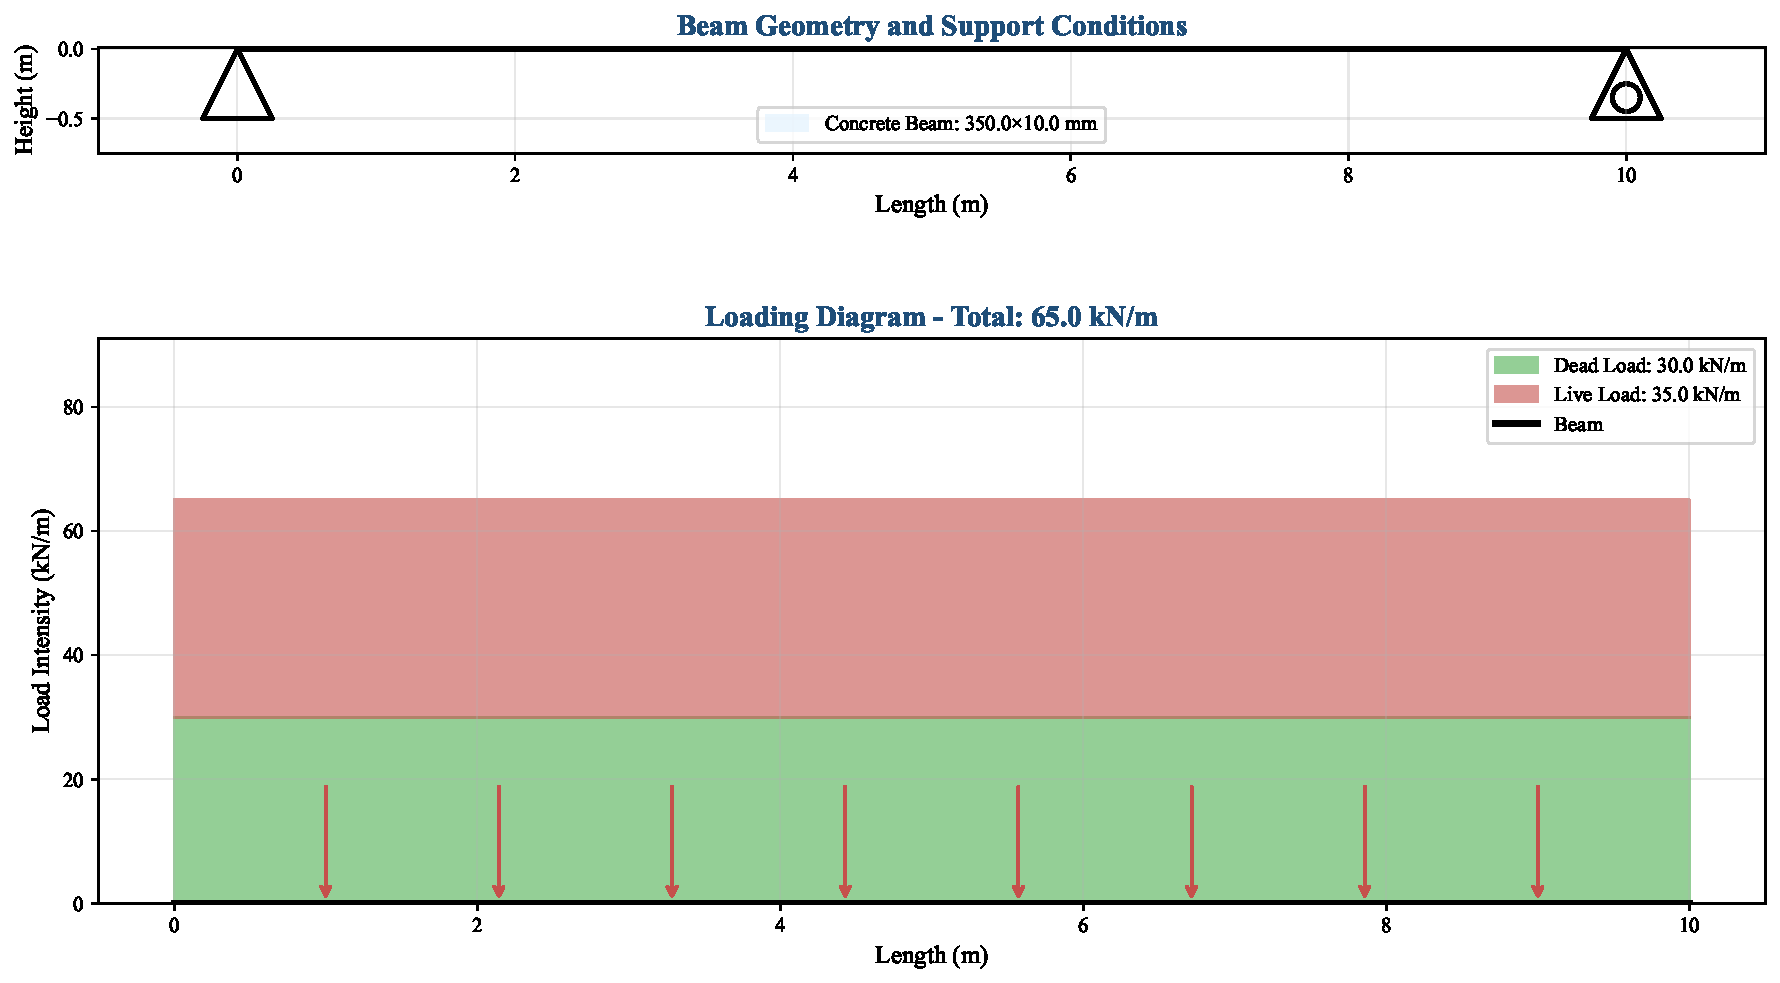
\includegraphics[width=\columnwidth]{beam_diagram.pdf}
\caption{Beam geometry and loading configuration}
\label{fig:beam_geometry}
\end{figure}

% Double column figure for BMD/SFD
\begin{figure*}[t]
\centering
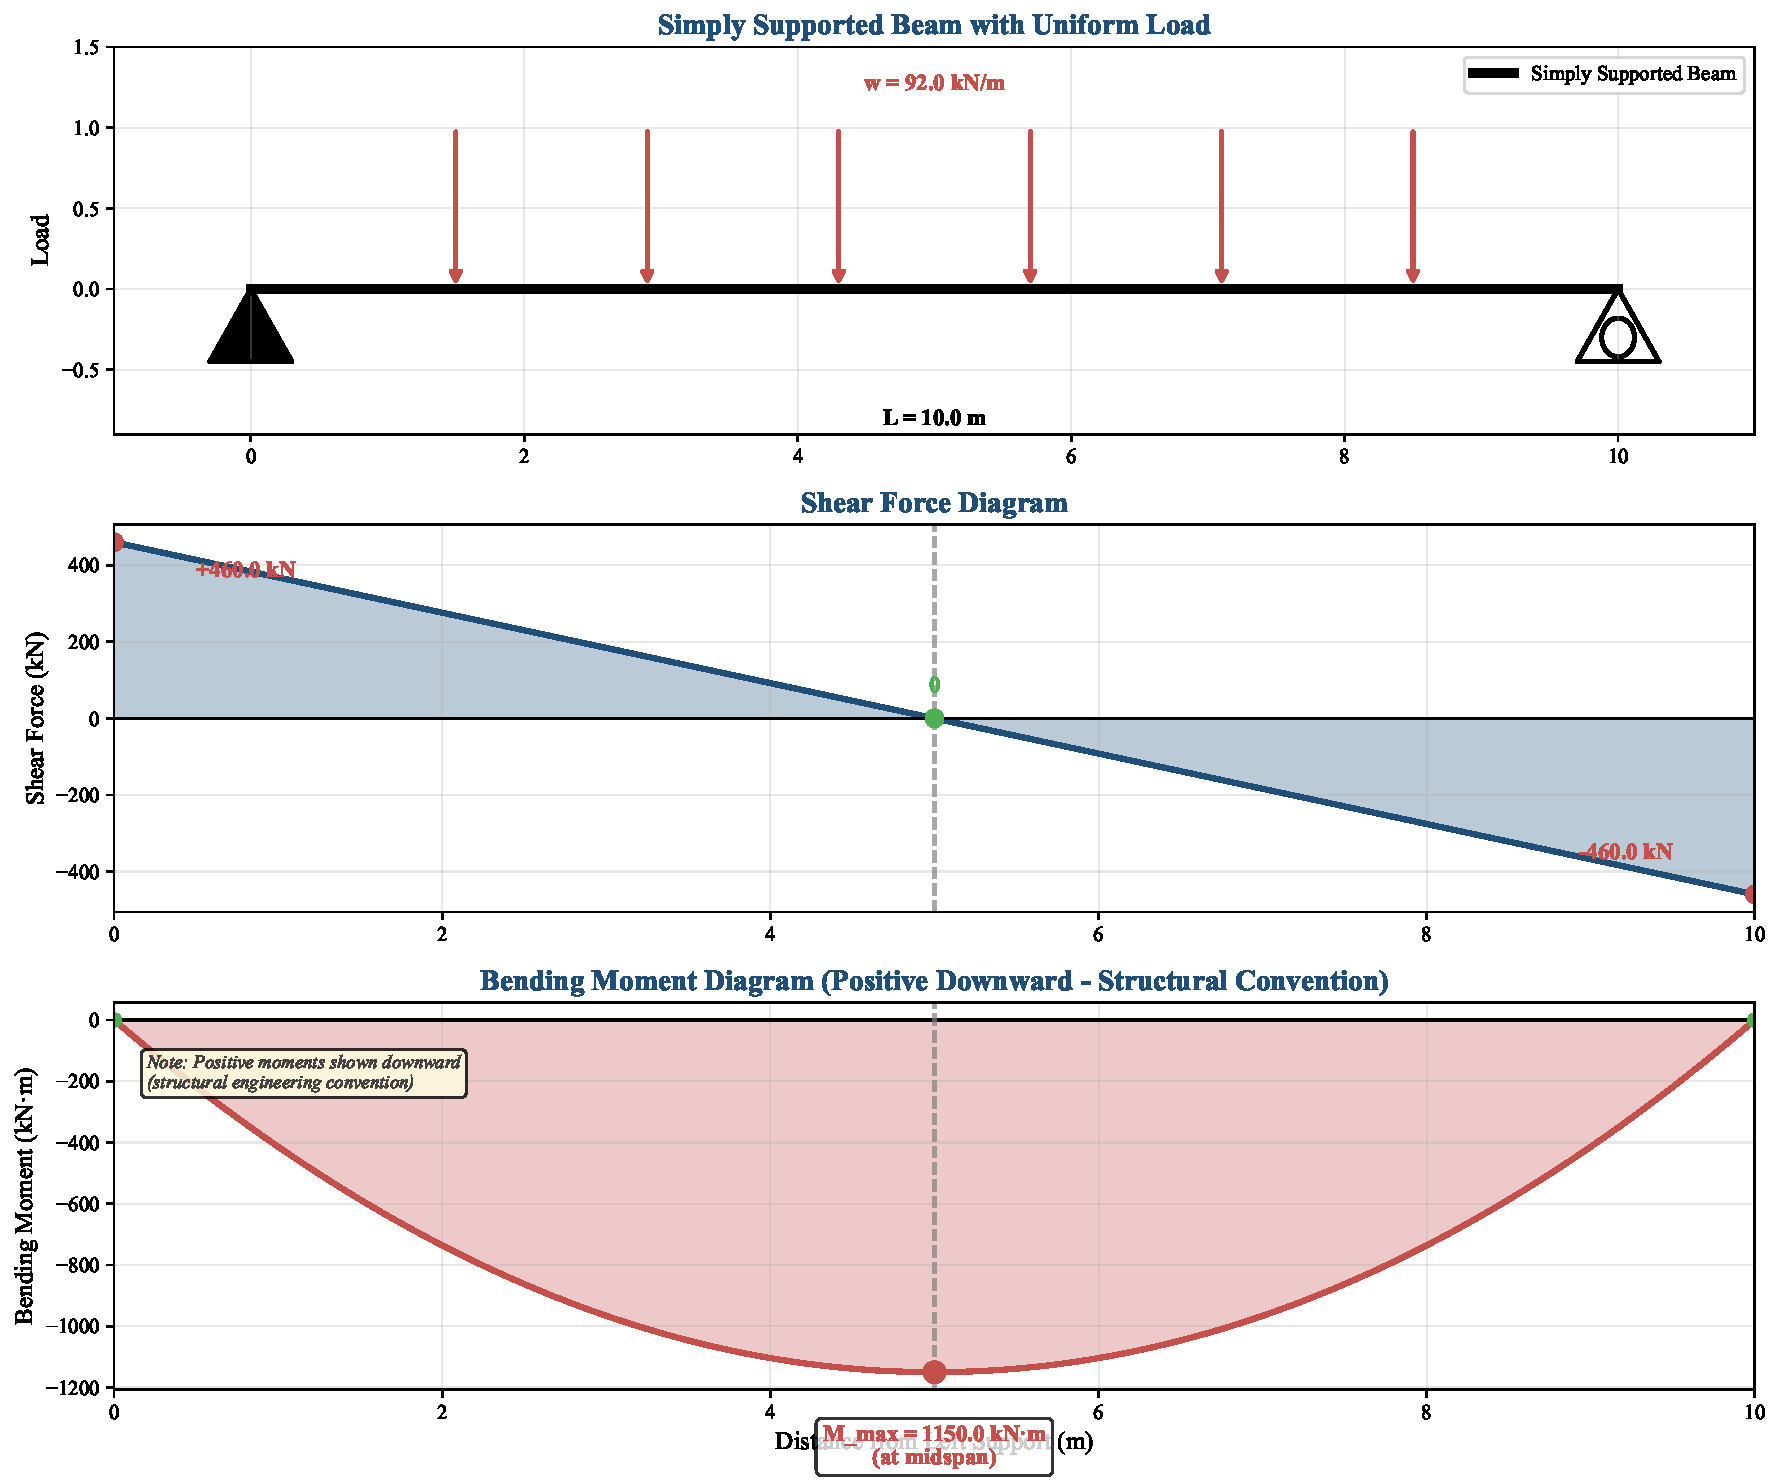
\includegraphics[width=0.8\textwidth]{bmd_sfd.pdf}
\caption{Bending moment and shear force diagrams (positive moments downward - structural engineering convention)}
\label{fig:bmd_sfd}
\end{figure*}

\begin{figure}[h]
\centering
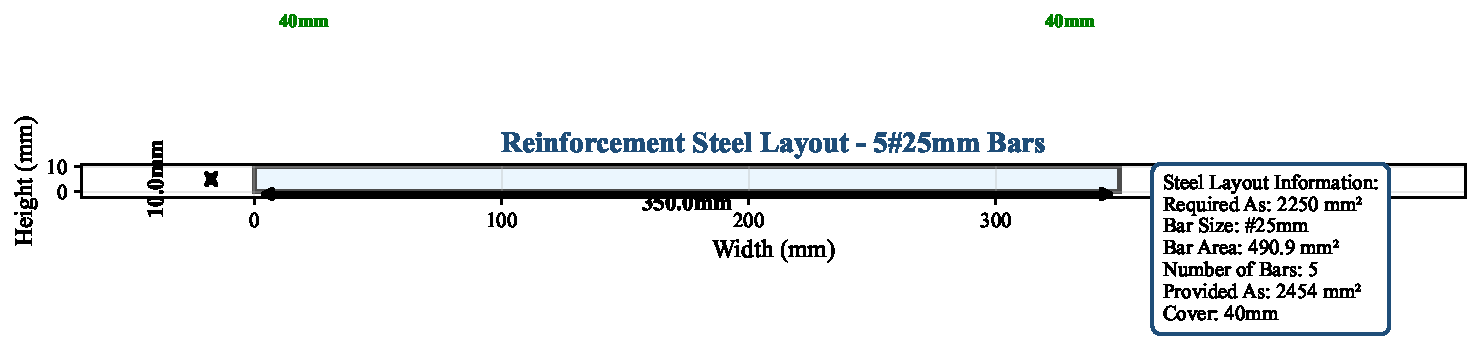
\includegraphics[width=\columnwidth]{steel_layout.pdf}
\caption{Reinforcement arrangement and detailing}
\label{fig:steel_layout}
\end{figure}

\section{Design Verification}

\subsection{Flexural Design}

The required flexural reinforcement is determined using strength design methodology per ACI 318-19 Section 22.2:

\begin{align}
A_{s,req} &= \frac{M_u}{\phi f_y (d - a/2)} \label{eq:steel_req}
\end{align}

where $\phi = 0.9$ is the strength reduction factor for flexure.

\subsection{Minimum Reinforcement}

Per ACI 318-19 Section 9.6.1.2, minimum reinforcement requirements ensure adequate ductility:

\begin{align}
A_{s,min} &= \max\left(\frac{0.25\sqrt{f'_c}}{f_y}bd, \frac{1.4}{f_y}bd\right) \label{eq:steel_min}
\end{align}

\subsection{Compliance Summary}

\begin{table}[h]
\centering
\caption{Design Compliance Verification}
\label{tab:compliance}
\begin{tabular}{@{}lcc@{}}
\toprule
\textbf{Requirement} & \textbf{Status} & \textbf{Reference} \\
\midrule
Flexural Capacity & \textcolor{ghaligreen}{\textbf{OK}} & ACI 22.2 \\
Minimum Steel & \textcolor{ghaligreen}{\textbf{OK}} & ACI 9.6.1.2 \\
Shear Capacity & \textcolor{ghaligreen}{\textbf{OK}} & ACI 22.5 \\
Serviceability & \textcolor{ghaligreen}{\textbf{OK}} & ACI 24.2 \\
\bottomrule
\end{tabular}
\end{table}

\section{Conclusion}

The reinforced concrete beam design has been completed in accordance with ACI 318-19 requirements. All structural capacity checks demonstrate adequate performance with appropriate safety factors. The tabulated format enables efficient analysis of multiple beam configurations with consistent methodology and professional presentation standards.

\paragraph{Key Features}
\begin{itemize}
\item Academic two-column format for efficient space utilization
\item Tabulated input/output system for multiple beam analysis
\item Professional engineering calculation methodology
\item Complete ACI 318-19 code compliance verification
\end{itemize}

% Professional signature block (academic style)
\begin{table}[h]
\centering
\caption*{Professional Certification}
\begin{tabular}{@{}cc@{}}
\toprule
\textbf{Prepared By} & \textbf{Reviewed By} \\
\midrule
Ahmed Ghali, P.E. & Senior Engineer, P.E. \\
Professional Engineer & Professional Engineer \\
Date: \today & Date: \_\_\_\_\_\_\_\_\_\_\_\_\_ \\
\bottomrule
\end{tabular}
\end{table}

% Bibliography section (Cambridge style)
\section*{References}

\begin{thebibliography}{9}
\bibitem{aci318}
ACI Committee 318. (2019). \textit{Building Code Requirements for Structural Concrete (ACI 318-19) and Commentary}. American Concrete Institute, Farmington Hills, MI.

\bibitem{maccormac}
MacCormac, J.C., \& Brown, R.H. (2016). \textit{Design of Reinforced Concrete: ACI 318-14 Code Edition}. John Wiley \& Sons.

\bibitem{nilson}
Nilson, A.H., Darwin, D., \& Dolan, C.W. (2015). \textit{Design of Concrete Structures}. McGraw-Hill Education.
\end{thebibliography}

\vspace{0.3cm}
{\scriptsize\textcolor{ghaligray}{
This calculation follows applicable engineering standards and professional practice guidelines. All calculations and results are subject to independent review and verification per professional engineering protocols.
}}

\end{document} 